\begin{quote}
    Diagram konečného stavového automatu (rozdelený na tri časti, kvôli prehľadnosti):
\end{quote}

\begin{figure}[!htbp]
    \centering
    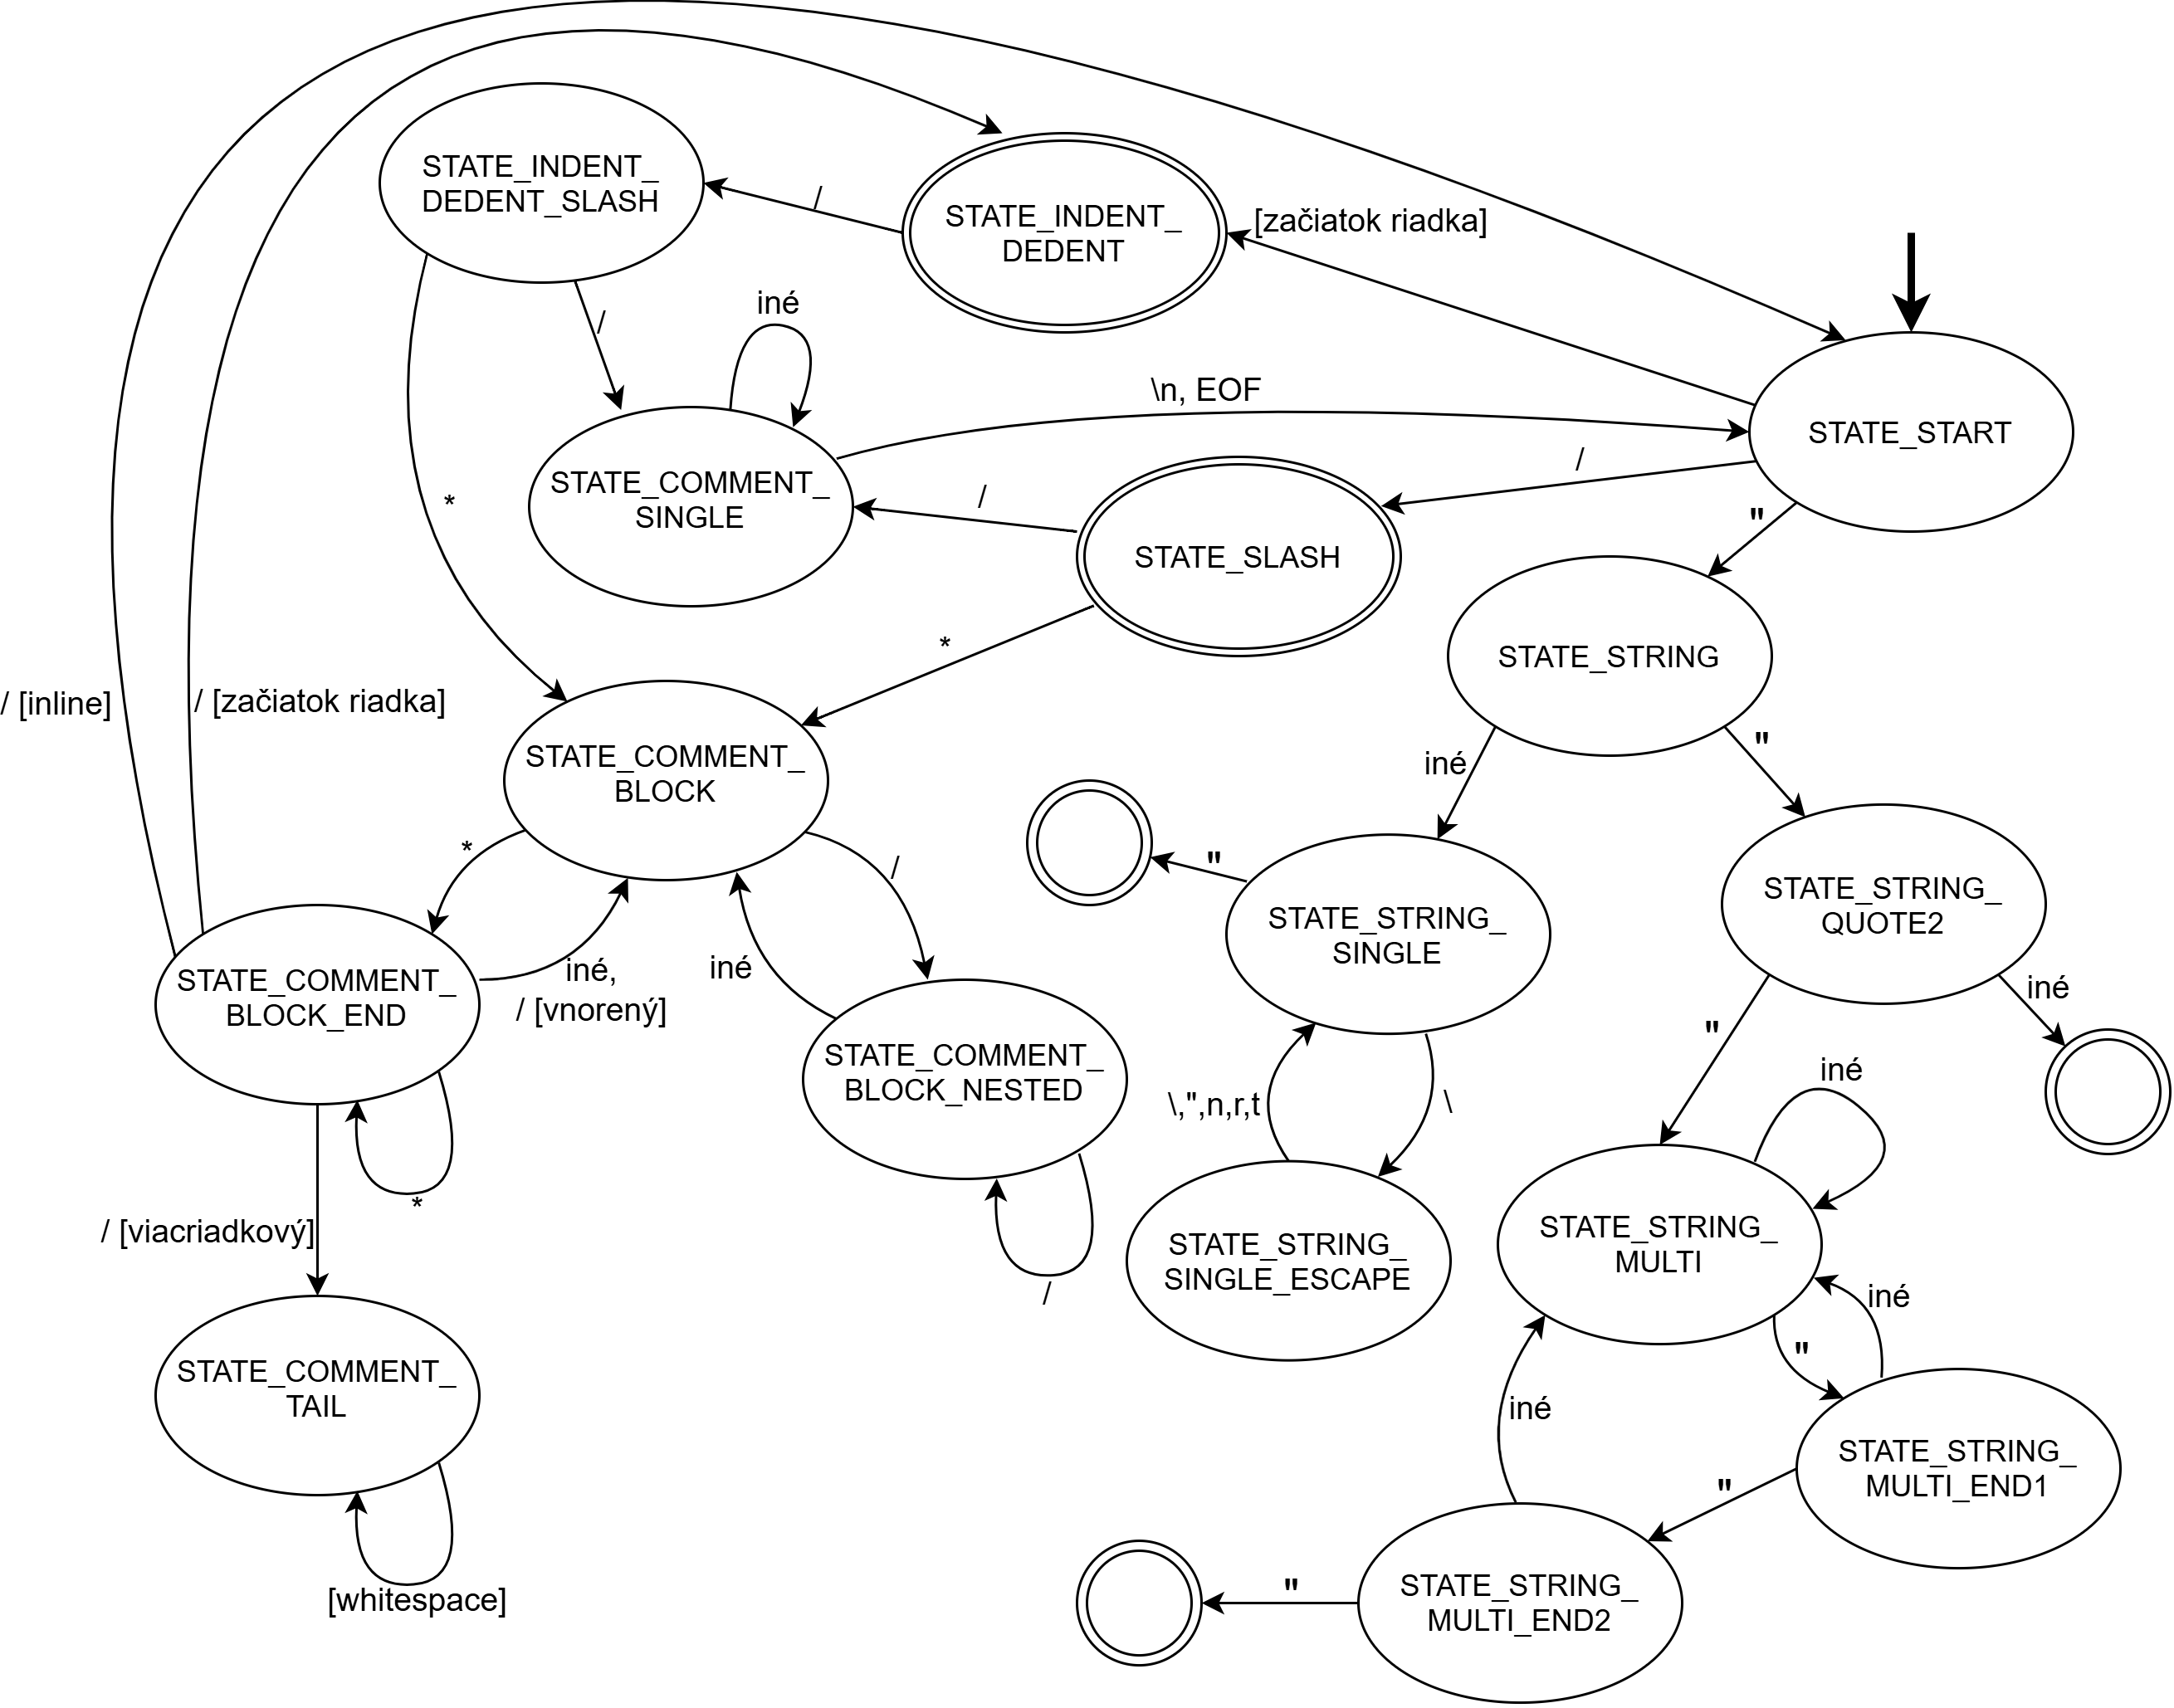
\includegraphics[width=0.97\textwidth, keepaspectratio]{images/indent,comment,string.png}
    \caption{Konečný stavový automat: stavy pre odsadenie, komentáre, textové reťazce}
\end{figure}

\vspace{1.4em}

\begin{figure}[!htbp]
    \centering
    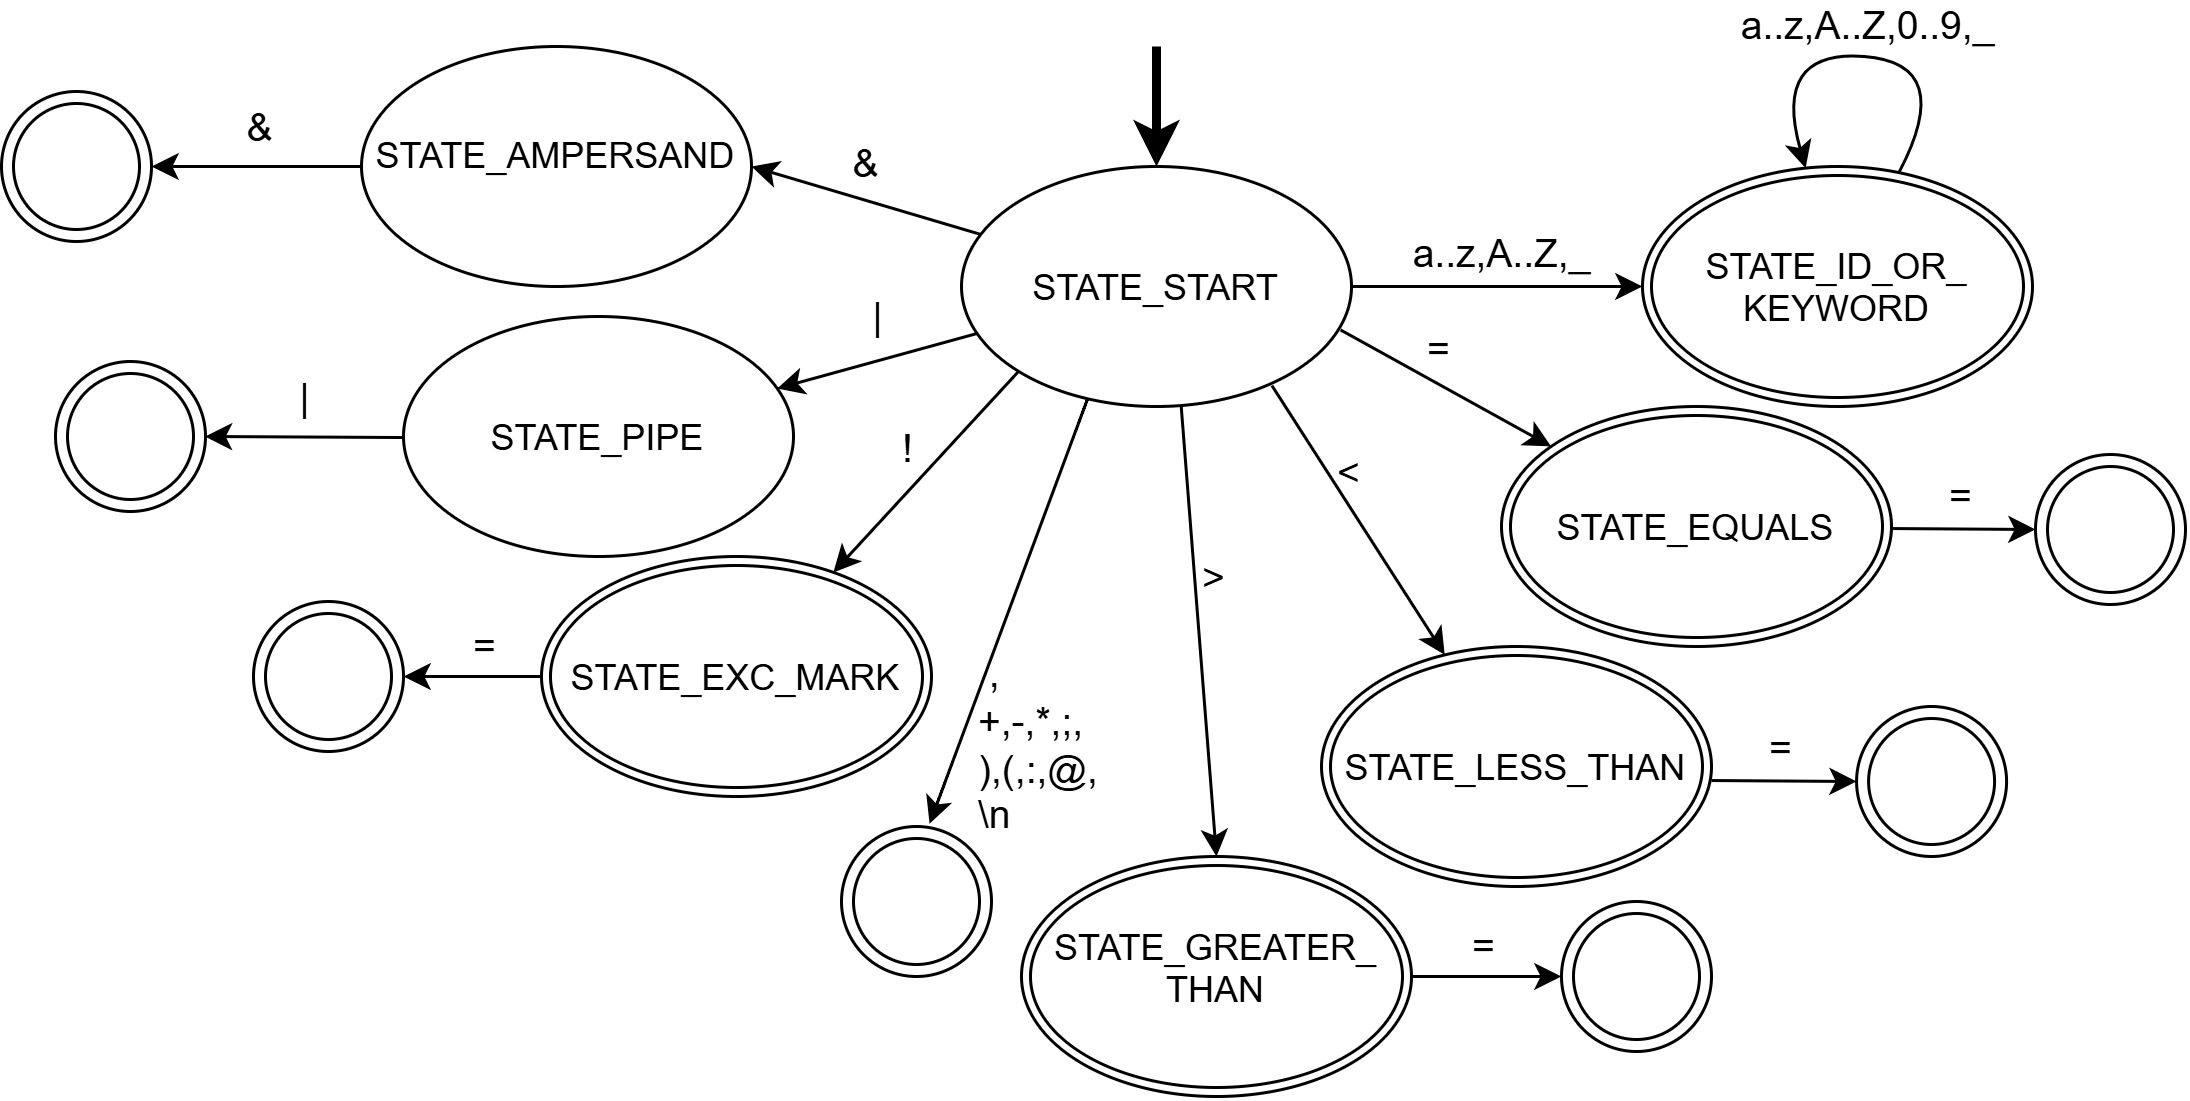
\includegraphics[width=0.85\textwidth, keepaspectratio]{images/keyword,simple.png}
    \caption{Konečný stavový automat: stavy pre operátory, oddeľovače, identifikátory a kľúčové slová}
\end{figure}


\begin{figure}[htbp]
    \centering
    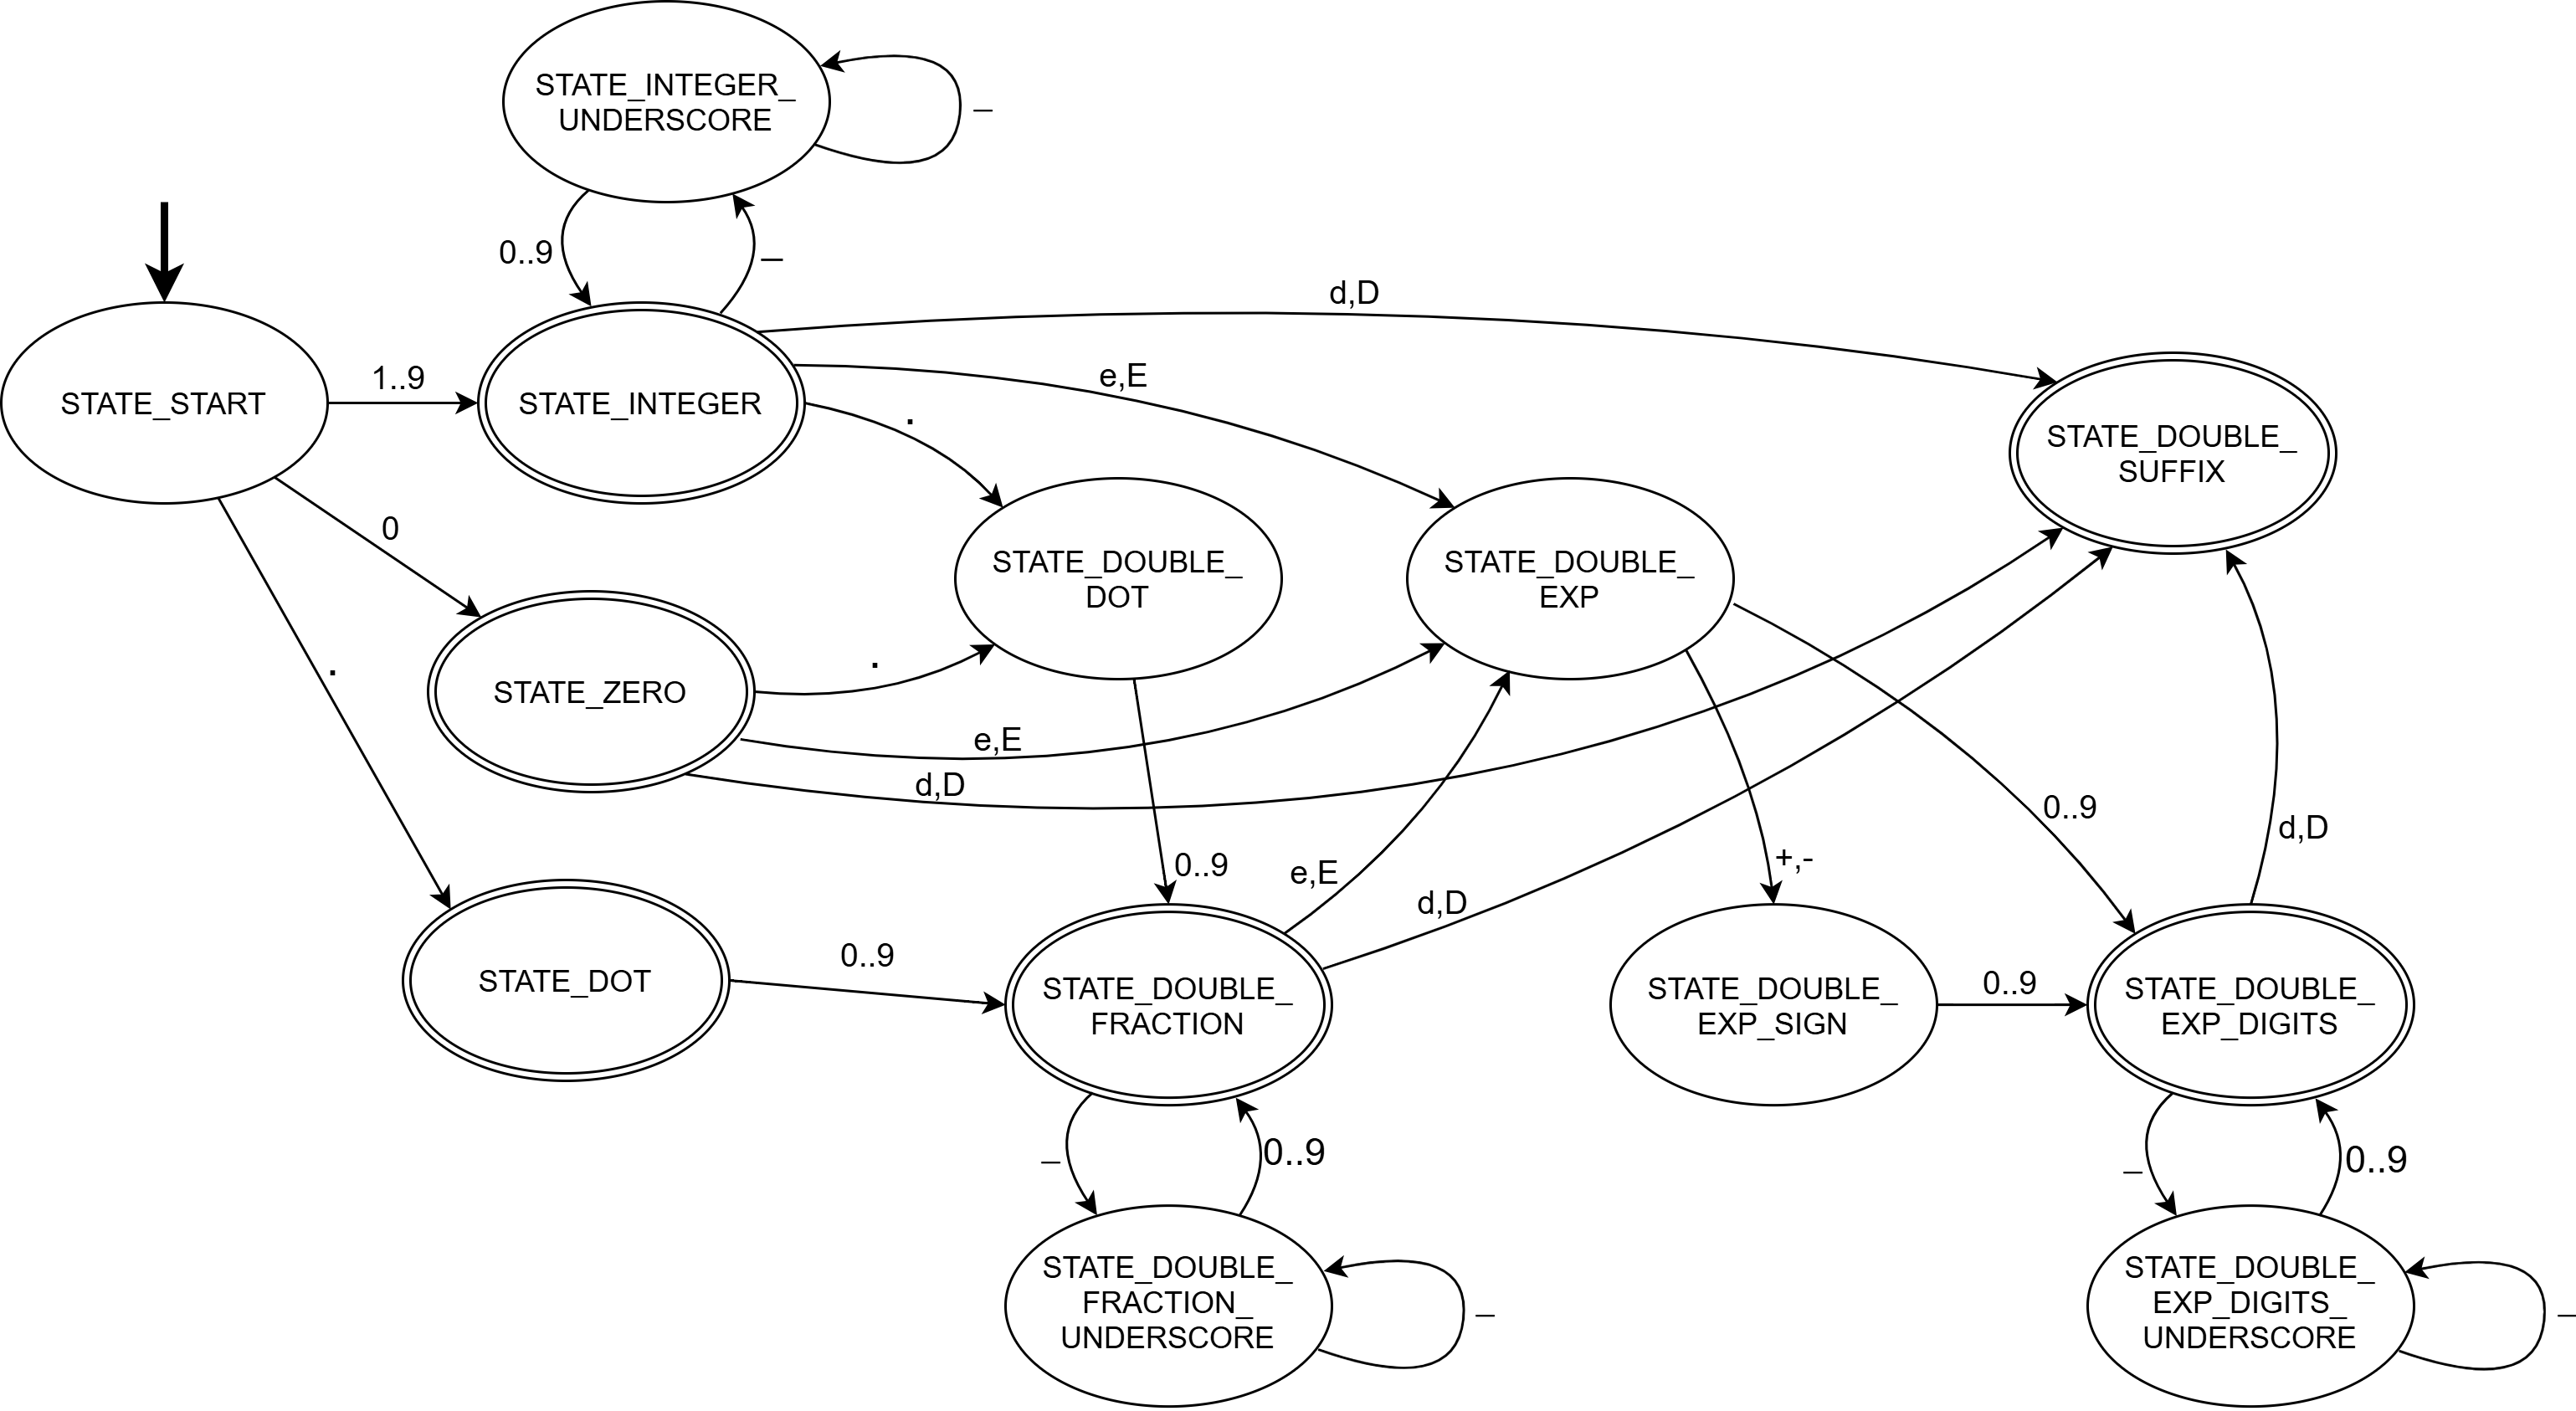
\includegraphics[width=1\textwidth, keepaspectratio]{images/int,double.png}
    \caption{Konečný stavový automat: stavy pre číselné literály}
\end{figure}


Odchýlky od klasického konečného stavového automatu:
\begin{itemize}
    \item V stave \texttt{INDENT\_DEDENT} a \texttt{INDENT\_DEDENT\_SLASH} sa neposielajú tokeny odsadenia hneď pri narazení na prvý nebiely znak v riadku, lebo nebielym znakom môže byť lomítko, a to môže znamenať začiatok komentára. Skener preto namiesto ďalšieho načítania znakov a prípadného dvojnásobného vrátenia znakov na vstup nastaví príznak, na základe ktorého sú vracané tokeny odsadenia mimo stavov automatu.
    \item Automat je \uv{zabalený} v ďalšej funkcii, ktorá filtruje tokeny tak, aby nikdy nebolo vrátených viac \texttt{EOL} tokenov po sebe. \texttt{EOL} je taktiež ignorovaný a nie je vracaný vnútri zátvoriek.
    \item Kľúčové slová a identifikátory nemajú samostatné stavy, sú rozlišované v jednom stave pomocou porovnávania stringu.
    \item Je využitých niekoľko počítadiel, ktoré ovplyvňujú prechody medzi stavmi. Tie sú uvedené v diagramoch v hranatých zátvorkách.
\end{itemize}


\newpage